\documentclass[11pt]{standalone}
\usepackage{color}
\usepackage[cmyk]{xcolor}
\usepackage{amsmath}
\usepackage{xltxtra}
\usepackage{libertine}

\usepackage{tikz}
\usetikzlibrary{intersections,arrows,calc}
% \tikzstyle{every picture}+=[thick]

\usepackage[active,tightpage]{preview}
\PreviewEnvironment{tikzpicture}
\setlength\PreviewBorder{1pt}%

\newcommand{\qbar}[1][b]{\kern 0.06em \overline{\kern -0.06em \text{#1} \kern -0.04em} \kern 0.04em}
\newcommand{\Bs}{\text{B}_\text{s}^\text{0}}
\newcommand{\kaon}[1][0]{\text{K}^\text{#1}}
\newcommand{\Kp}{\kaon[+]}
\newcommand{\Km}{\kaon[--]}
\newcommand{\pimes}[1][]{\text{π}^\text{#1}}
\newcommand{\lmu}[1][]{\text{μ}^\text{#1}}
\newcommand{\nul}[1][]{\text{ν}_\text{#1}}
\newcommand{\nulbar}[1][]{\kern 0.04em \overline{\kern -0.04em \nul[#1] \kern -0.25em} \kern 0.25em}
\newcommand{\numubar}{\nulbar[μ]}

\begin{document}
\sffamily
\begin{tikzpicture}
  \node[anchor=south]{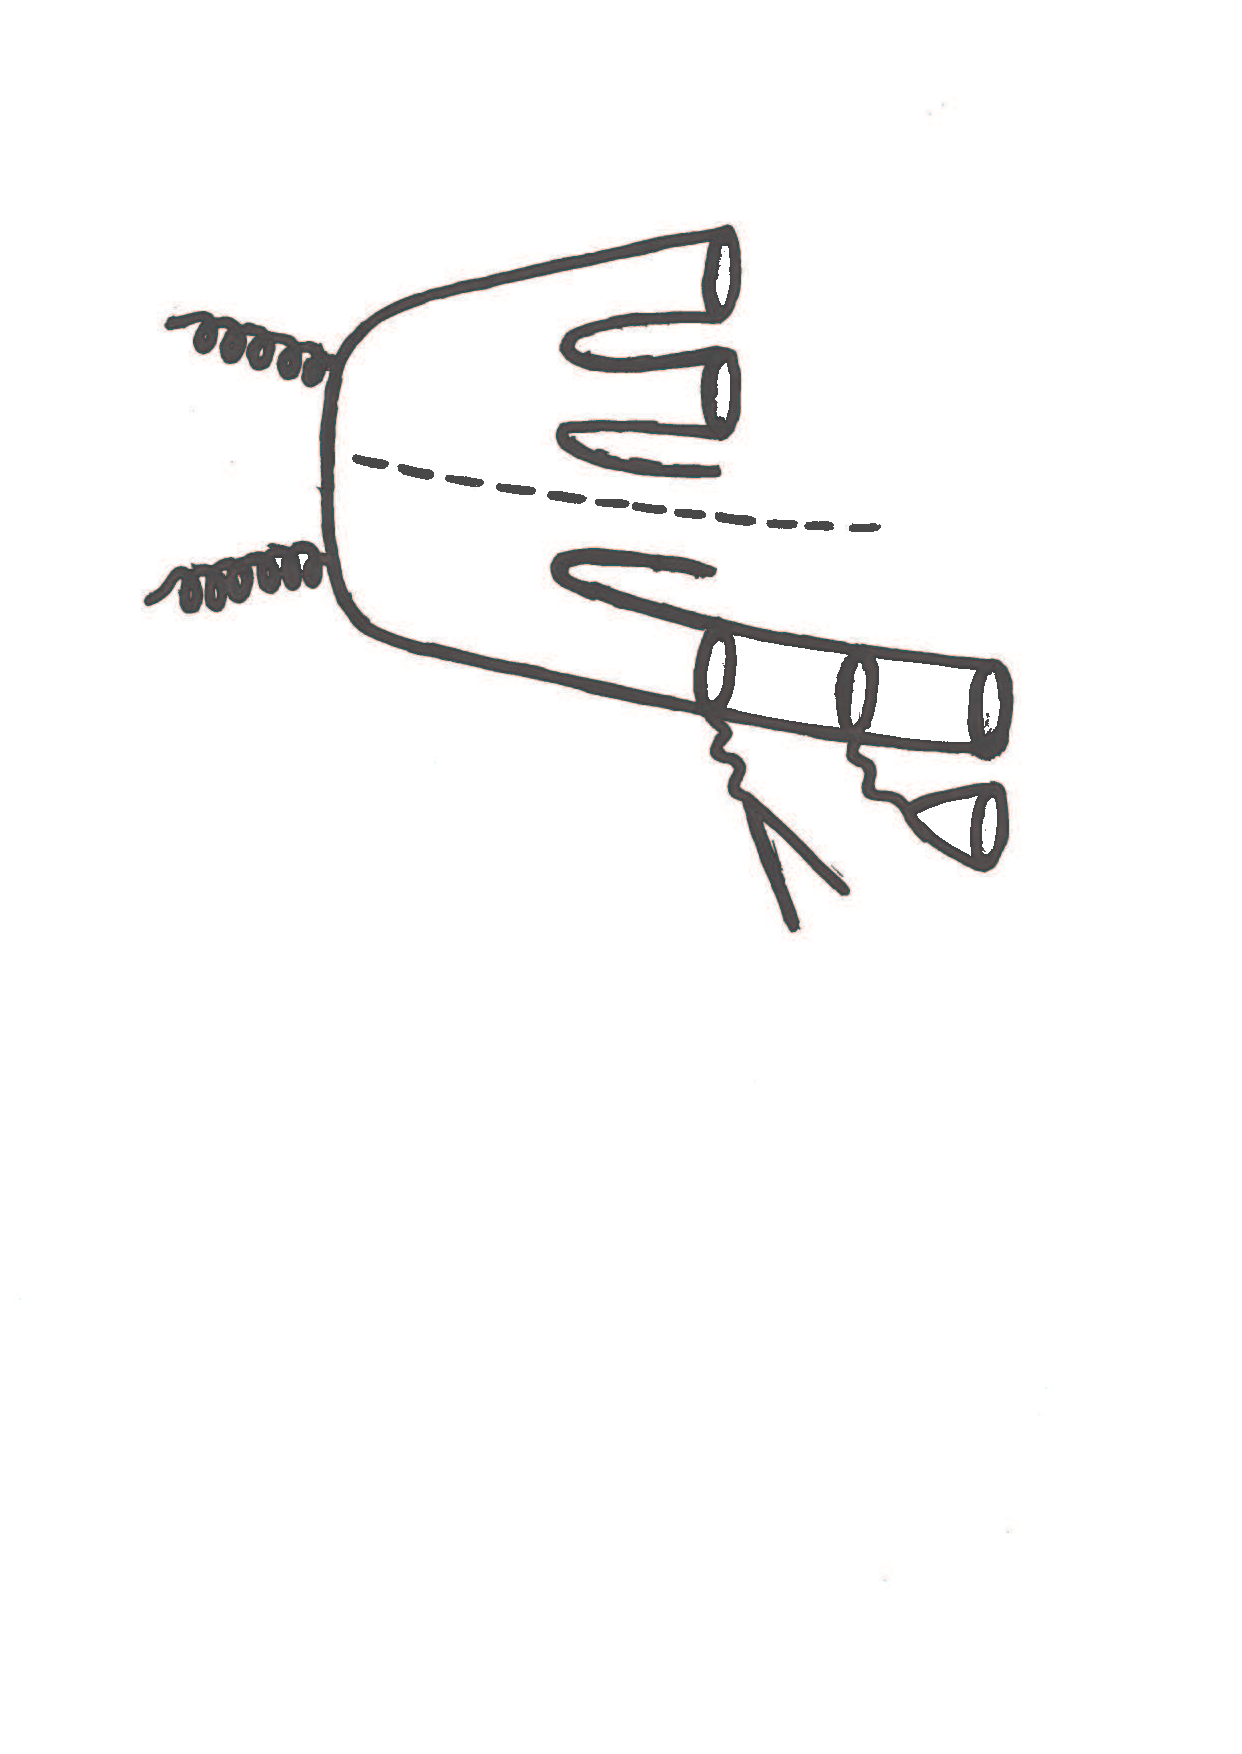
\includegraphics[clip=true, trim=22mm 137mm 36mm 36mm, width=0.55\textwidth]{../tagging_CMYK}};
  %\draw[help lines] (-4,0) grid (4,7);
  \node at ( -1.43,  2.18 ) {b};
  \node at ( -1.43,  5.43 ) {$\qbar[b]$};
  \node at ( -0.40,  5.00 ) {s};
  \node at ( -0.40,  4.68 ) {$\qbar[s]$};
  \node at ( -0.42,  4.22 ) {u};
  \node at ( -0.42,  3.89 ) {$\qbar[u]$};
  \node at ( -0.46,  3.22 ) {u};
  \node at ( -0.46,  2.89 ) {$\qbar[u]$};
  \node at (  1.62,  1.60 ) {c};
  \node at (  2.60,  1.49 ) {s};
  \node at (  1.70,  5.34 ) {$\Bs$};
  \node at (  1.70,  4.46 ) {$\Kp$};
  \node at (  3.80,  1.98 ) {$\Km$};
  \node at (  3.80,  1.13 ) {$\pimes[+]$};
  \node at (  1.85, -0.14 ) {$\lmu[--]$};
  \node at (  2.44,  0.28 ) {$\numubar$};
\end{tikzpicture}
\end{document}
